\chapter{The Language of Motion}\label{ch:02_language_of_motion}

\begin{laymansbox}{Why We Need a Language}{box:ch02_language}

A statement such as ``the hips turn early'' leaves several questions open: which body rotates relative to which frame, which angle describes that rotation, and early relative to what event? Mathematics helps us answer those questions only after we define the quantities. An equation with an unspecified angle can be just as ambiguous as a coaching phrase.

This chapter builds a description of motion from configuration, velocity and state. We then connect joint motion to the motion of a distal endpoint. These distinctions matter because a useful golf model must explain both how the body moves and what the club delivers at impact. A precise motion description is the beginning of that investigation; it does not by itself identify the forces or the control strategy.

\end{laymansbox}

\section{Coordinates: Measuring Position}\label{ch02:coordinates-measuring-position}

\subsection{Cartesian Coordinates and Body Orientation}\label{ch02:cartesian-coordinates-and-body-orientation}

\protect\phantomsection\label{ch02:cartesian-coordinates}{}

A point in space has Cartesian coordinates \((x,y,z)\) relative to a stated origin and three perpendicular axes. These describe that point's location. They do not describe an entire club: two clubs can put the same point at the same location with different face orientations. A rigid body's configuration generally needs both position and orientation.

Coordinates are descriptions, not physical causes. Changing from laboratory coordinates to joint coordinates does not change the motion. It changes the numbers and the equations used to describe it. Mixing numbers from different frames or angle conventions does change the calculation, usually incorrectly.

\subsection{Generalized Coordinates and Degrees of Freedom}\label{ch02:generalized-coordinates-and-degrees-of-freedom}

\protect\phantomsection\label{ch02:generalized-coordinates}{}

A configuration specifies the positions and orientations of the modeled bodies, without their velocities. In a regular local description, \textbf{independent generalized coordinates} \(\bm q=(q_1,\ldots,q_n)\) parameterize that configuration using \(n\) variables. This local number is the configuration's number of degrees of freedom (DOF).

A single coordinate chart need not cover every configuration without a seam or singularity. An angle and that angle plus \(2\pi\) describe the same orientation of an ideal revolute hinge. We can unwrap an angle along a motion, but the unwrapped number also records turns. Alternatively, redundant coordinates can be useful if their constraints are enforced; Cartesian coordinates are not an inferior choice.

For an ideal planar pendulum with a fixed pivot and rigid link of length \(L\),

\[
x=L\sin\theta,\qquad y=-L\cos\theta,\qquad x^2+y^2=L^2.
\]

One angle suffices even though we wrote two position components. This assumes motion confined to a plane. A spherical pendulum free to swing in space has two configuration DOF. A string gives a fixed-distance constraint only while taut; it cannot supply the compressive force a rigid rod can. These are different physical models.

\subsection{A Declared Two-Link Model}\label{ch02:a-declared-two-link-model}

We will use the same geometric model as Chapter~\ref{ch:03_double_pendulum}: two rigid links in a fixed inertial plane, a fixed base pivot \(O\), a connecting hinge \(H\), and distal endpoint \(P\). There are two ideal revolute joints and no joint limits in this baseline.

The labels ``shoulder'' and ``elbow'' can be helpful analogies, but they do not make this an anatomical arm model. Interpreting the hinge as an elbow differs from interpreting it as an arm--club connection. We therefore use link 1, link 2 and hinge throughout. A real swing adds moving supports, three-dimensional orientation, both arms, compliant structures and contact.

Use horizontal \(x\) positive to the right and vertical \(y\) positive upward. The first angle \(\theta_1\) increases counterclockwise from downward vertical. The second angle \(\theta_2\) is the counterclockwise \textbf{relative} angle from link 1 to link 2. Thus

\[
\bm q=\begin{bmatrix}\theta_1\\\theta_2\end{bmatrix},
\qquad \alpha_1=\theta_1,\qquad \alpha_2=\theta_1+\theta_2.
\]

The \(\alpha_i\) are absolute link angles in the plane. Earlier notation \(\theta_s,\theta_e\) corresponds to \(\theta_1,\theta_2\) only under this declared idealization; it is not a pair of measured anatomical rotations. At \(\bm q=(0,0)\) both links hang downward. Zero does not mean pointing toward a golf target.

\begin{figure}[htbp]
\centering
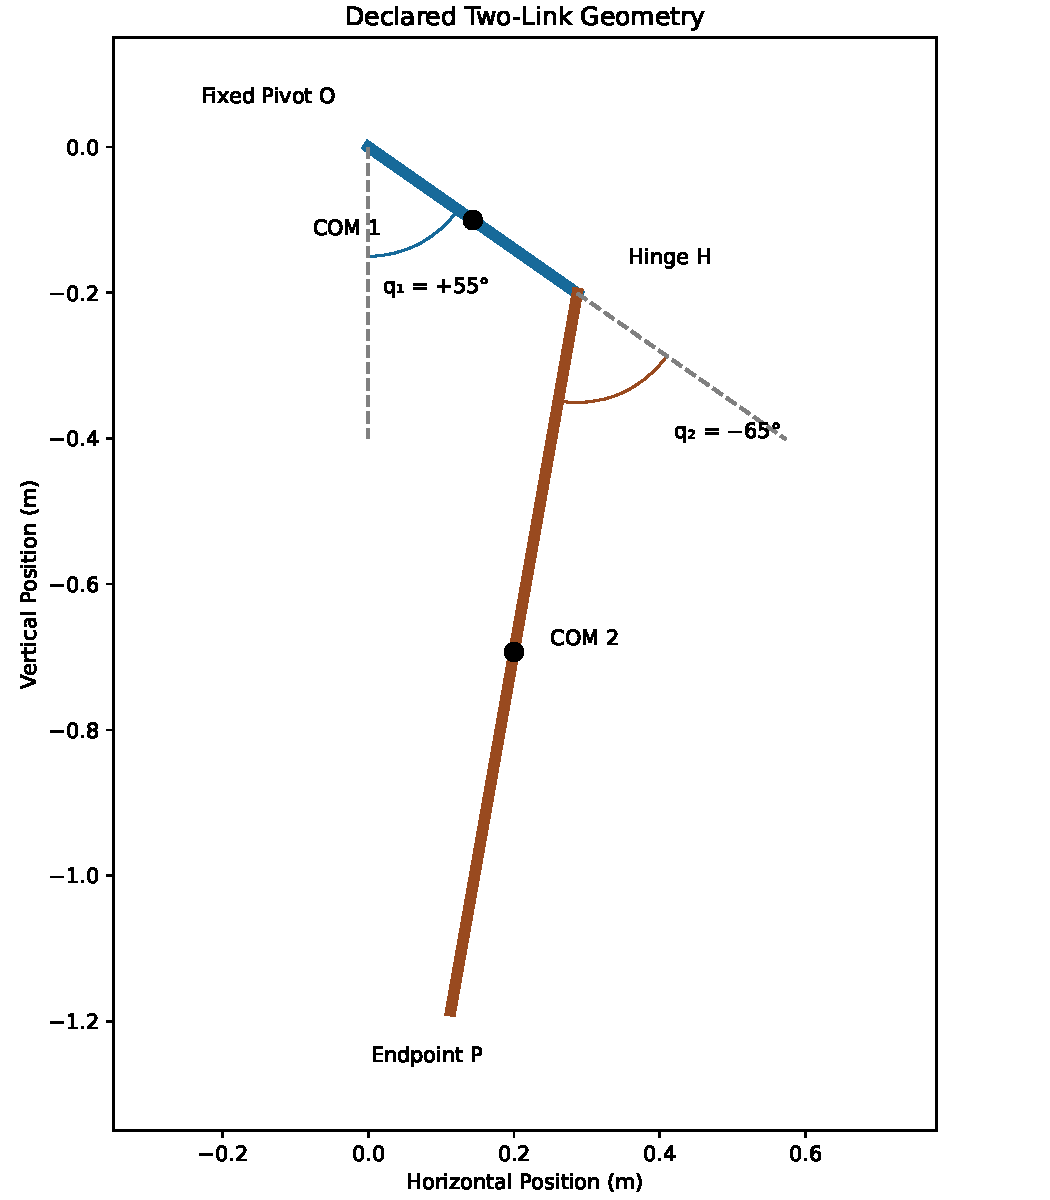
\includegraphics[width=0.85\linewidth,height=0.6\textheight,keepaspectratio]{figures/double_pendulum_verified.pdf}
\caption{Two-Link Coordinate Convention. The Computed Geometry Is Shared With Chapter 3; It Illustrates a Model, Not Measured Golf Anatomy.}
\label{fig:ch02_arm_diagram}
\end{figure}

\section{Configuration Space and Constraints}\label{ch02:configuration-space-and-constraints}

\protect\phantomsection\label{ch02:configuration-space-the-space-of-positions}{}

\subsection{A Map of Configurations}\label{ch02:a-map-of-configurations}

For unrestricted revolute joints, the two angles each lie on a circle. Their product is a torus. A square plot of angles is a useful map of this configuration space, provided opposite edges are identified: crossing an angle seam is not a physical jump.

Joint limits or collision exclusions remove configurations from this ideal space. A rectangular angle window can illustrate chosen independent limits; it is not a universal map of human shoulder and elbow motion. Anatomical limits depend on the joint definition, other joint positions, loading and the individual. We do not infer them from the ideal model.

This distinction between a space and its coordinates is developed in the \href{https://modernrobotics.northwestern.edu/nu-gm-book-resource/2-3-1-configuration-space-topology/}{Modern Robotics configuration-space treatment}. The important practical question is what the chosen coordinates represent and where that representation remains valid.

\subsection{Admissibility Is Not Reachability}\label{ch02:admissibility-is-not-reachability}

\protect\phantomsection\label{ch02:constraints-not-all-configurations-are-allowed}{}

A configuration can satisfy geometric constraints yet be unreachable from a specified starting state with the available torques, time and contact conditions. \textbf{Admissibility} concerns the declared constraints. \textbf{Dynamic reachability} also depends on the initial state, equations, input bounds and elapsed time.

For example, a link arrangement may be geometrically possible while a requested transition to it in 20 ms exceeds the model's actuator bounds. The number 20 ms here defines a hypothetical request, not a measured human capability. Configuration space alone cannot decide whether the transition can be performed.

\subsection{Position, Velocity and Contact Constraints}\label{ch02:position-velocity-and-contact-constraints}

\protect\phantomsection\label{ch02:constraints-in-the-double-pendulum-model}{} \protect\phantomsection\label{box:ch02_golf_constraints}{}

A smooth equality constraint \(h(\bm q)=0\) whose Jacobian has independent rows restricts configuration. Differentiating it gives the compatible velocity condition

\[
\bm H(\bm q)\dot{\bm q}=0,\qquad
\bm H=\frac{\partial h}{\partial\bm q}.
\]

Some velocity constraints cannot be integrated into position constraints. Rolling without slipping is a standard example. It limits instantaneous motion without necessarily reducing configuration dimension. The \href{https://modernrobotics.northwestern.edu/nu-gm-book-resource/2-4-configuration-and-velocity-constraints/}{Modern Robotics constraint treatment} distinguishes these holonomic and nonholonomic cases.

For the two-link baseline, using hinge angles already enforces rigid attachment; we need not add another equation to hold the hinge together. If instead we modeled each body's free Cartesian pose, attachment would appear as explicit constraints. The same physical reaction can therefore be implicit in one formulation and explicit in another.

Real grip and ground contacts require a declared contact mode. Sticking is possible only when the required contact forces and moments lie within the model's admissible contact set. Feet remaining in place do not freeze every torso coordinate, and a held club does not eliminate wrist motion. Slip, separation and changing contact patches can change the equations.

\subsection{What a Constraint Reaction Means}\label{ch02:what-a-constraint-reaction-means}

\protect\phantomsection\label{box:ch02_constraints_walls}{}

In an ideal constrained model, a reaction is solved together with the acceleration to enforce compatible motion. It is not generally a freely chosen actuator input. Nevertheless, changing muscle or actuator forces can change that reaction. Mathematical classification as a reaction does not identify which tissues carry the physical load.

A hard joint stop is one possible idealization. Biological resistance can involve passive tissue deformation, active muscle forces and rate-dependent effects before a nominal range limit is reached. Replacing that response with an impenetrable wall does not predict tissue loading or injury. Chapter~\ref{ch:constraint_forces} develops the force balance and work assumptions more carefully.

\section{State: What Is Needed to Predict Motion?}\label{ch02:state-what-is-needed-to-predict-motion}

\protect\phantomsection\label{ch02:state-position-and-velocity}{}

\subsection{Velocity and Its Units}\label{ch02:velocity-and-its-units}

\protect\phantomsection\label{ch02:angular-velocity}{} \protect\phantomsection\label{ch02:ref-Nesbit2005}{} \protect\phantomsection\label{ch02:ref-Hume2005}{}

The generalized velocity is the time derivative \(\dot{\bm q}\). For an angle, its units are radians per second. Degrees may be useful for reporting values, but differentiation of sine and cosine in the formulas below assumes radians.

For illustration, a planar link rotating at \(500^\circ/\mathrm{s}\) has angular speed \(500\pi/180\approx8.727\) rad/s. At fixed radius 0.35 m, a point on that link has speed about 3.054 m/s. This is a unit conversion and rigid-link calculation, not a typical measured shoulder rate.

In this planar model, \(\omega_1=\dot\theta_1\) and \(\omega_2=\dot\theta_1+\dot\theta_2\). In a general three-dimensional model, the derivatives of three orientation coordinates are not simply the three components of angular velocity; a representation-dependent map is required.

\subsection{A State Belongs to a Specified Model}\label{ch02:a-state-belongs-to-a-specified-model}

For a smooth, unconstrained, second-order mechanical model with independent coordinates, a convenient state is

\[
\bm x=
\begin{bmatrix}\bm q\\\dot{\bm q}\end{bmatrix},
\qquad
\dot{\bm x}=
\begin{bmatrix}\dot{\bm q}\\\bm a(t,\bm q,\dot{\bm q},\bm u)\end{bmatrix}.
\]

The acceleration function \(\bm a\) comes from a declared dynamic model; \(\bm u\) denotes its inputs. An initial state, model parameters and future input history or feedback rule define an initial-value problem. Standard regularity and existence assumptions are also needed for a unique solution. Knowing only the instantaneous forces supplies instantaneous acceleration, not all future commands.

Position alone cannot distinguish passing through a configuration quickly from resting there. Conversely, zero velocity at one instant does not tell us whether motion will reverse, remain at rest or accelerate onward; the model and inputs decide.

The \(2n\) state dimension is appropriate to this mechanical model, not to every biological model. Muscle activation, tendon or shaft deformation, controller memory and other internal variables may require additional states. Delay models can require a history rather than a finite list of instantaneous values. Contacts add modes and compatibility conditions. A video-derived joint configuration is therefore not automatically a complete predictive state.

\begin{laymansbox}{A State Is More Than a Pose}{box:ch02_state}

Imagine two swings with the same visible link arrangement. Different rates already make their futures different. Even matching those rates may be insufficient if stored elastic deformation, muscle activation or the upcoming control inputs differ. State selection is a modeling commitment about what information is enough to advance the equations.

\end{laymansbox}

\section{Phase Space and Trajectories}\label{ch02:phase-space-and-trajectories}

\protect\phantomsection\label{ch02:phase-space-where-every-swing-lives}{}

For the unconstrained two-link baseline, \(\bm x=(\theta_1,\theta_2,\dot\theta_1,\dot\theta_2)\) has four components locally. The velocity at a configuration can take many values: configuration does not assign one unique velocity arrow. A tangent vector \((\dot\theta_1,\dot\theta_2)\) lies in the tangent space at a configuration; the full state-space direction is \((\dot{\bm q},\ddot{\bm q})\).

Here phase space means the position--velocity state space (the tangent bundle of configuration space). Hamiltonian mechanics instead uses positions and conjugate momenta; a nonsingular mechanical Legendre map relates these descriptions. Neither convention adds a new physical motion.

A \textbf{trajectory} is a time-parameterized state history. Its configuration projection forgets the velocities. A plot of \((\theta_1,\dot\theta_1)\) forgets the second joint, so it is a projection, not a slice fixing the omitted variables. Projected curves can cross without the full states being equal. Even full-state uniqueness concerns the same time-dependent model and input rule; different commands need not produce the same continuation.

For smooth motion, configuration and velocity evolve continuously. An ideal impulsive impact can leave position continuous while resetting velocity. Hybrid state histories are then piecewise smooth with jumps, rather than one everywhere-smooth curve. The moment at which the club reaches a ball also matters: comparing two swings at the same clock time differs from comparing them at their respective impact events.

\section{From Joint Motion to Endpoint Motion}\label{ch02:from-joint-motion-to-endpoint-motion}

\subsection{Positions and Centers of Mass}\label{ch02:positions-and-centers-of-mass}

\protect\phantomsection\label{ch02:position-kinematics}{}

Write the radial and tangent directions as

\[
\bm e(\alpha)=\begin{bmatrix}\sin\alpha\\-\cos\alpha\end{bmatrix},
\qquad
\bm t(\alpha)=\frac{d\bm e}{d\alpha}
=\begin{bmatrix}\cos\alpha\\\sin\alpha\end{bmatrix}.
\]

With link lengths \(L_1,L_2\) and COM distances \(r_1,r_2\) from their proximal hinges,

\[
\begin{aligned}
\bm r_H&=L_1\bm e(\theta_1),\\
\bm r_P&=L_1\bm e(\theta_1)+L_2\bm e(\theta_1+\theta_2),\\
\bm r_{\mathrm{COM},1}&=r_1\bm e(\theta_1),\\
\bm r_{\mathrm{COM},2}&=L_1\bm e(\theta_1)+r_2\bm e(\theta_1+\theta_2).
\end{aligned}
\]

These are planar positions in the declared fixed frame. A specified embedding can place that plane in three-dimensional space; two coordinates still do not reconstruct unrestricted spatial arm or club motion. The COM need not be at half the link length, and the distal endpoint need not be the COM.

For the examples here use \(L_1=0.35\) m, \(L_2=1.0\) m, \(r_1=0.175\) m and \(r_2=0.5\) m. These are the manufactured geometric parameters of Chapter 3. Kinematics does not require masses. When dynamics is added, that chapter supplies masses 2.5 kg and 0.4 kg and separate centroidal inertias. These numbers do not calibrate a golfer.

\subsection{The Jacobian Is a Directional Map}\label{ch02:the-jacobian-is-a-directional-map}

\protect\phantomsection\label{ch02:velocity-kinematics}{}

Differentiating the endpoint position gives

\[
\dot{\bm r}_P=\bm J_P(\bm q)\dot{\bm q},
\]

\[
\bm J_P=
\begin{bmatrix}
L_1\cos\theta_1+L_2\cos(\theta_1+\theta_2)&L_2\cos(\theta_1+\theta_2)\\
L_1\sin\theta_1+L_2\sin(\theta_1+\theta_2)&L_2\sin(\theta_1+\theta_2)
\end{bmatrix}.
\]

Each column gives endpoint velocity per unit rate of one coordinate while the other rate is zero. The columns add with their signed rates. Describing a matrix as ``large'' is incomplete: specify the input-rate direction and norm, and the output direction or speed being compared.

At \(\bm q=(0,0)\),

\[
\bm J_P=\begin{bmatrix}1.35&1.0\\0&0\end{bmatrix}.
\]

Rates \((1,-1.35)\) rad/s give zero instantaneous endpoint velocity; \((1,1.35)\) rad/s give 2.7 m/s to the right. The same geometry can produce cancellation or reinforcement. Neither calculation alone measures mechanical advantage, required torque or available power.

The determinant is \(L_1L_2\sin\theta_2\). At aligned links the endpoint velocity map loses rank, although both joint coordinates still exist. This task singularity does not by itself make the mass matrix singular. Angular-rate addition is kinematics; inertial coupling depends on the mass distribution and kinetic energy derived in Chapter 3.

\subsection{Acceleration and a Moving Support}\label{ch02:acceleration-and-a-moving-support}

Another derivative introduces a term even when joint accelerations vanish:

\[
\ddot{\bm r}_P=\bm J_P\ddot{\bm q}+\dot{\bm J}_P\dot{\bm q},
\]

\[
\dot{\bm J}_P\dot{\bm q}
=-L_1\dot\theta_1^2\bm e(\theta_1)
-L_2(\dot\theta_1+\dot\theta_2)^2\bm e(\theta_1+\theta_2).
\]

These terms account for the changing velocity directions as links rotate. They are accelerations, not individual muscle forces. The \href{https://underactuated.mit.edu/multibody.html}{MIT multibody derivation} provides the corresponding relative-angle kinematics and mechanical formulation.

If the pivot translates while the plane's axes remain inertially fixed, add \(\dot{\bm r}_O\) to endpoint velocity and \(\ddot{\bm r}_O\) to endpoint acceleration. If the coordinate frame also rotates, differentiating that frame adds further terms. A fixed-pivot model cannot silently represent the effects of a moving hand path or turning torso.

\section{A Consistent Manufactured Trajectory}\label{ch02:a-consistent-manufactured-trajectory}

\protect\phantomsection\label{ch02:phase-space-portrait-of-a-swing}{}

Replace an assumed ``typical swing'' table with a differentiable example whose signs can be checked. Let \(T=0.5\) s and \(s=t/T\) for \(0\leq t\leq T\):

\[
\theta_1=\frac{\pi}{2}(1-s^2),\qquad
\theta_2=-\frac{\pi}{4}(1-s).
\]

\[
\dot\theta_1=-\frac{\pi}{T}s,\qquad
\dot\theta_2=\frac{\pi}{4T},\qquad
\ddot\theta_1=-\frac{\pi}{T^2},\qquad \ddot\theta_2=0.
\]

\begin{center}
\small
\begin{tabular}{rrrrr}
\toprule
$t$ (s)&$\theta_1$ (deg)&$\theta_2$ (deg)&$\dot\theta_1$ (deg/s)&$\dot\theta_2$ (deg/s)\\
\midrule
0&90&-45&0&90\\
0.25&67.5&-22.5&-180&90\\
0.5&0&0&-360&90\\
\bottomrule
\end{tabular}
\end{center}

This is an illustrative segment, not measured golf data or a full address-to-follow-through swing. At its start, the first coordinate has a turning point while the second link is already rotating. At its end, both links point downward, but the state differs from rest. There is no assumed ball collision at that endpoint.

The same values can be reproduced directly:

\begin{lstlisting}[language=Python,breaklines=true,basicstyle=\ttfamily\footnotesize]
# Manufactured Chapter 2 trajectory
import numpy as np

duration_s = 0.5
time_s = np.array([0.0, 0.25, 0.5])
phase = time_s / duration_s
q_deg = np.column_stack((90 * (1 - phase**2), -45 * (1 - phase)))
rate_deg_s = np.column_stack((-180 * phase / duration_s, np.full(3, 45 / duration_s)))
q_rad = np.deg2rad(q_deg)
rate_rad_s = np.deg2rad(rate_deg_s)
\end{lstlisting}

At \(t=T\), substitution into the Jacobian gives

\[
\dot{\bm r}_P=
\begin{bmatrix}-2.2\pi\\0\end{bmatrix}\ \mathrm{m/s}
\approx\begin{bmatrix}-6.912\\0\end{bmatrix}\ \mathrm{m/s}.
\]

The acceleration is \((-5.4\pi,\,3.65\pi^2)\) m/s\(^2\): leftward tangential and upward normal components. This makes the interplay explicit: configuration sets the velocity map, signed rates set the current motion and curvature terms, and joint accelerations supply the remaining acceleration.

A fully actuated ideal model with invertible inertia and unrestricted input moments can realize this smooth segment by inverse dynamics. That statement supplies no evidence that a human can realize it with physiological limits, contact constraints or the intended impact task. Those are additional questions.

\section{From Motion to Forces and Golf Outcomes}\label{ch02:from-motion-to-forces-and-golf-outcomes}

\protect\phantomsection\label{ch02:from-coordinates-to-forces}{}

Forward dynamics uses the model, state and inputs to compute acceleration. Inverse dynamics uses a sufficiently differentiated motion, inertial parameters and external-load assumptions to compute required net generalized forces. It generally does not determine a unique set of individual muscle, grip or ground forces. Multiple load distributions can produce the same generalized effect.

For a useful golf investigation, define the task as well as the state. Clubhead position and speed do not specify face orientation, contact location or ball launch. Earlier forces and energy exchanges influence the state arriving near impact; posture and rates determine the instantaneous kinematic map; inertia and feasible inputs constrain what can change before contact. Ground and grip conditions influence those feasible inputs. A contact model then relates the arriving club and ball states to the collision outcome.

This is why the aspects must be studied together. Kinematics supplies the geometry of motion; dynamics supplies the force and energy balance; control specifies how inputs are chosen; measurements test whether the chosen model and explanations match a golfer. None of these layers can substitute for the others.

\begin{principle}{Key Takeaways}{pr:ch02_key_takeaways}

\begin{enumerate}
\def\labelenumi{\arabic{enumi}.}

\item
  Declare the body, frame, angle reference and sign before interpreting a coordinate.
\item
  Configuration dimension, admissible velocity dimension and predictive state dimension are different questions.
\item
  A complete state is complete for a specified model and future input rule.
\item
  The Jacobian maps signed rates to task velocity; acceleration also includes changing-geometry terms.
\item
  Constraint reactions depend on the equations and loading. Their mathematical role does not identify individual tissues or guarantee feasible contact.
\item
  A consistent synthetic example checks reasoning; it does not establish human performance or a coaching prescription.
\end{enumerate}

\end{principle}

\section{Chapter Exercises With Worked Answers}\label{ch02:chapter-exercises-with-worked-answers}

\protect\phantomsection\label{ch02:chapter-exercises}{}

\subsection*{1. Count the Configuration and Velocity Dimensions}\label{ch02:count-the-configuration-and-velocity-dimensions}

Consider a planar rigid pendulum, a spherical rigid pendulum, an unrestricted planar two-link chain, and an oriented sphere rolling without slipping on a horizontal plane. State the assumptions.

\textbf{Answer.} Their configuration dimensions are 1, 2, 2 and 5 respectively. For the sphere, two numbers locate the center in the plane and three specify orientation. With radius \(R\) and angular velocity \(\bm\omega\), zero velocity at the contact point gives

\[
v_x=R\omega_y,\qquad v_y=-R\omega_x.
\]

There are three freely selectable instantaneous velocity components, not five: two independent no-slip conditions constrain the five configuration rates. Spin \(\omega_z\) remains allowed by this ideal point-contact condition. Forbidding spin is an additional assumption. Ignoring orientation changes the question to locating the center rather than describing the full rigid-body configuration.

A human upper-body count cannot be inferred from the words ``shoulder, elbow and wrist'' alone. A declared open chain with a 3-DOF shoulder, 1-DOF elbow and 2-DOF wrist has six configuration DOF at a fixed base. Adding forearm rotation, a second arm or closed grasp constraints changes that model and requires a new count.

\subsection*{2. Draw the Configuration Map}\label{ch02:draw-the-configuration-map}

Draw a square \((-\pi,\pi]\times(-\pi,\pi]\) for the ideal two-link chain and identify opposite edges. Add an illustrative restriction \(|\theta_2|\leq\pi/2\).

\textbf{Answer.} The unrestricted square represents a torus, not four physical walls. The added restriction removes configurations with larger relative angles; it does not establish a human range limit or guarantee that every remaining point is reachable within a prescribed time and torque budget.

\subsection*{3. Calculate a Point Speed}\label{ch02:calculate-a-point-speed}

For \(L_1=0.35\) m and \(\dot\theta_1=500^\circ/\mathrm{s}\), find hinge speed with the base fixed.

\textbf{Answer.} Convert to radians first: \(|\dot{\bm r}_H|=0.35(500\pi/180)\approx3.054\) m/s. At \(\theta_1=0\) the positive-rate velocity points right; at \(\theta_1=\pi/2\) it points up. These are signs in the declared frame, not target-relative swing directions.

\subsection*{4. Distinguish Endpoint Velocity From Acceleration}\label{ch02:distinguish-endpoint-velocity-from-acceleration}

At \(\bm q=(0,0)\) and rates \((1,0)\) rad/s, set both joint accelerations to zero.

\textbf{Answer.} Endpoint velocity is \((1.35,0)\) m/s, but acceleration is \((0,1.35)\) m/s\(^2\). Zero joint angular acceleration does not mean zero Cartesian acceleration. The velocity direction is changing.

\subsection*{5. Interpret a Phase Projection}\label{ch02:interpret-a-phase-projection}

Can two points with identical \((\theta_1,\dot\theta_1)\) have different endpoint velocities?

\textbf{Answer.} Yes. With rates \((1,0)\) rad/s, configurations \((0,0)\) and \((0,\pi/2)\) give endpoint velocities \((1.35,0)\) and \((0.35,1)\) m/s. The projection has discarded the second angle. In the manufactured trajectory, a zero first-coordinate rate at \(t=0\) likewise does not imply a motionless endpoint: its speed is \(\pi/2\) m/s.

\subsection*{6. Interpret a Limit Without Inventing Physiology}\label{ch02:interpret-a-limit-without-inventing-physiology}

A model imposes a rigid joint stop. What changes if tissue compliance is modeled instead?

\textbf{Answer.} An ideal reaction enforces the stop's compatibility conditions, potentially with an impact law at engagement. A compliant model allows deformation and requires a force--deformation--rate law and any internal states it uses. Actuation can affect the load in either formulation. Neither formulation alone establishes a person's safe range or predicts injury.

\section{On This Site}\label{ch02:on-this-site}

\protect\phantomsection\label{ch02:related-reading}{}

\protect\phantomsection\label{ch02:quarto-bibliography}{}

Continue with Chapter~\ref{ch:03_double_pendulum}, Chapter~\ref{ch:constraint_forces}, and Chapter~\ref{ch:inverse_dynamics_parallel}. For spatial descriptions, see \href{https://affinedrift.com/articles/rotation-representations-reference.html}{rotation representations}; for model size, see \href{https://affinedrift.com/articles/degrees-of-freedom-and-dimensionality.html}{degrees of freedom and dimensionality}. The site's \href{https://affinedrift.com/pages/notation.html}{notation reference} supplies the broader conventions; each model must still declare its particular frame and input definitions.
